\documentclass{article}

\usepackage[margin=3cm]{geometry}

\geometry{a4paper,left=2cm,right=2cm,top=2.54cm,bottom=2.54cm}
%加這個就可以設定字體
\usepackage{fontspec}
    % 普通文字,行距
        \usepackage[onehalfspacing]{setspace}
    
    % 段落間距  (begin doc 才設定)
        \usepackage{parskip}
%使用xeCJK,其他的還有CJK或是xCJK
    % 中文
    \usepackage{xeCJK}
    \setCJKmainfont[AutoFakeBold=3]{DFKai-SB} %设置中
    \usepackage[fontsize=14pt]{fontsize}
% 首行縮排距離
    \setlength\parindent{28pt}
        % 首行縮排
        \usepackage{indentfirst}

%%%%%%%%%%%%%%%%%%%%%%%%
%%%%    三、圖片
%%%%%%%%%%%%%%%%%%%%%%%%


    %%%%    啟用圖片功能
    \usepackage{graphicx}

    %%%%    設定圖片路徑
    \graphicspath{ {./img/} }

    %%%%    設定圖片定位
    \usepackage{float}

    %%%%    把Figure變成"圖"
    \renewcommand{\figurename}{Fig}

%%%%%%%%%%%%%%%%%%%%%%%%
%%%%%%%              end

% 目錄顯示層次
    \setcounter{tocdepth}{2}
% 計算
\usepackage{enumitem}

%設定英文字型,不設的話就會使用預設的字型
\setmainfont{Times New Roman}

\usepackage{fontspec}
\usepackage{titlesec}
\usepackage{graphicx}
\usepackage{physics}
\usepackage{amsmath}
\usepackage{mathtools}
\usepackage{setspace}
\usepackage{subfigure} %所需宏包

\usepackage[hidelinks]{hyperref}
 \usepackage{titlesec}
    % 定义section格式,包括中文数字
   
    \usepackage{zhnumber}
\titleformat{\section}
  {\fontsize{18pt}{15}\bfseries}
  {\selectfont\thesection.}
  {0.5em}
  {}

\usepackage{fancyhdr}
\pagestyle{fancy}

\usepackage{color, xcolor}

\usepackage{algorithm}
\usepackage{algpseudocode}


% New definitions
\algnewcommand\algorithmicswitch{\textbf{switch}}
\algnewcommand\algorithmiccase{\textbf{case}}
\algnewcommand\algorithmicassert{\texttt{assert}}
\algnewcommand\Assert[1]{\State \algorithmicassert(#1)}%
% New "environments"
\algdef{SE}[SWITCH]{Switch}{EndSwitch}[1]{\algorithmicswitch\ #1\ \algorithmicdo}{\algorithmicend\ \algorithmicswitch}%
\algdef{SE}[CASE]{Case}{EndCase}[1]{\algorithmiccase\ #1}{\algorithmicend\ \algorithmiccase}%
\algtext*{EndSwitch}%
\algtext*{EndCase}%

\usepackage{newfloat}
\DeclareFloatingEnvironment[
  fileext = lol ,
  listname = {List Of Listings} ,
  name = Listing
]{listing}

\makeatletter
\newenvironment{breakablealgorithm}
  {% \begin{breakablealgorithm}
    \footnotesize
   \begin{center}
     \refstepcounter{algorithm}% New algorithm
     \hrule height.8pt depth0pt \kern2pt% \@fs@pre for \@fs@ruled
     \renewcommand{\caption}[2][\relax]{% Make a new \caption
       {\raggedright\textbf{\ALG@name~\thealgorithm} ##2\par}%
       \ifx\relax##1\relax % #1 is \relax
         \addcontentsline{loa}{algorithm}{\protect\numberline{\thealgorithm}##2}%
       \else % #1 is not \relax
         \addcontentsline{loa}{algorithm}{\protect\numberline{\thealgorithm}##1}%
       \fi
       \kern2pt\hrule\kern2pt
     }
  }{% \end{breakablealgorithm}
     \kern2pt\hrule\relax% \@fs@post for \@fs@ruled
   \end{center}
  }
\makeatother

\usepackage{pdfpages}
\algnewcommand\And{\textbf{and}}
\algnewcommand\Or{\textbf{or}}

\usepackage{amsmath}

\newcommand\mycommfont[1]{\footnotesize\ttfamily\textcolor{mygreen}{#1}}

\usepackage{tikz, ifthen}
\usetikzlibrary{calc,shapes, positioning,chains,arrows}

\usepackage{everyshi}  % 用于在每一页应用浮水印


% 畫底線
\usepackage{ulem}


\definecolor{myblue}{HTML}{6B73D5}
\definecolor{myred}{HTML}{C00000}
\definecolor{myyellow}{HTML}{FFDB57}

\usepackage[hidelinks]{hyperref}
\hypersetup{urlcolor=myblue, % url
citecolor=black, % citation
linkcolor=black, % table of contents, inner color
colorlinks=true, }
\usepackage{enumitem}

\usepackage{listings}

\definecolor{Blue}{rgb}{0,0,1}
\definecolor{Green}{rgb}{0,0.5,0}
\definecolor{Red}{rgb}{0.64,0.08,0.08}


\lstset{
    captionpos=t,                       % 讓Caption在Bottom的位置
    numbers=left,                       % 程式碼行號
    frame=single,
    showstringspaces=false,             % "不"標註空格
    escapeinside={(*@}{@*)},            % 脫逃字元
    commentstyle=\color{Green},         % Comment顏色
    keywordstyle=\color{Blue},          % Keyword顏色
    stringstyle=\color{Red},            % String顏色
    basicstyle=\ttfamily\scriptsize,         % 字型
    breaklines = true,
}


\begin{document}



\thispagestyle{empty}

\begin{center}
        \vspace*{3cm} %垂直距離
        {\Huge\bf
            \underline{CAD for VLSI Design }\\}%\uppercase\expandafter{\romannumeral 1}}
        \vspace{3cm}
        {\bf\huge Project Assignment 2\\}
        \vspace{0.5cm}
        {\bf\fontsize{23pt}{20}\selectfont Partitioning\\}
        \vspace{4cm}
        {\fontsize{23pt}{26pt} \selectfont Instructor: Andy, Yu-Guang Chen  Ph.D.\\}
        {\fontsize{20pt}{26pt} \selectfont TA: Yi-Ting Lin\\}
        \vspace{2cm}
        \fontsize{22pt}{25pt}\selectfont
        Department/Class: Electrical Engineering 4A\\
        \vspace*{1em}
        Name: {\bf 陳緯亭}\\
        \vspace*{1em}
        Student ID Number: {\bf 109501201}\\
\vspace{2cm}
\end{center}
\newpage


\tableofcontents
\listoflistings


\thispagestyle{empty}
\newpage


 \setcounter{page}{1}

 \lhead{109501201\ 陳緯亭}

% --------------------------------------------------------


\section{How I compile and execute the program}

\begin{figure}[H]
  \centering
  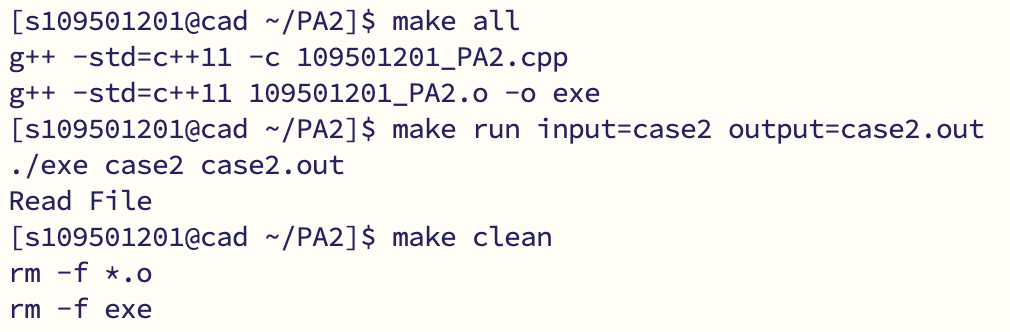
\includegraphics[width=\linewidth]{./img/2024-04-23-12-39-30.png}
  \caption{Using make to compile and execute
  my program}
  \label{g++}
\end{figure}

\vspace*{-1em}

\begin{figure}[H]
  \centering
  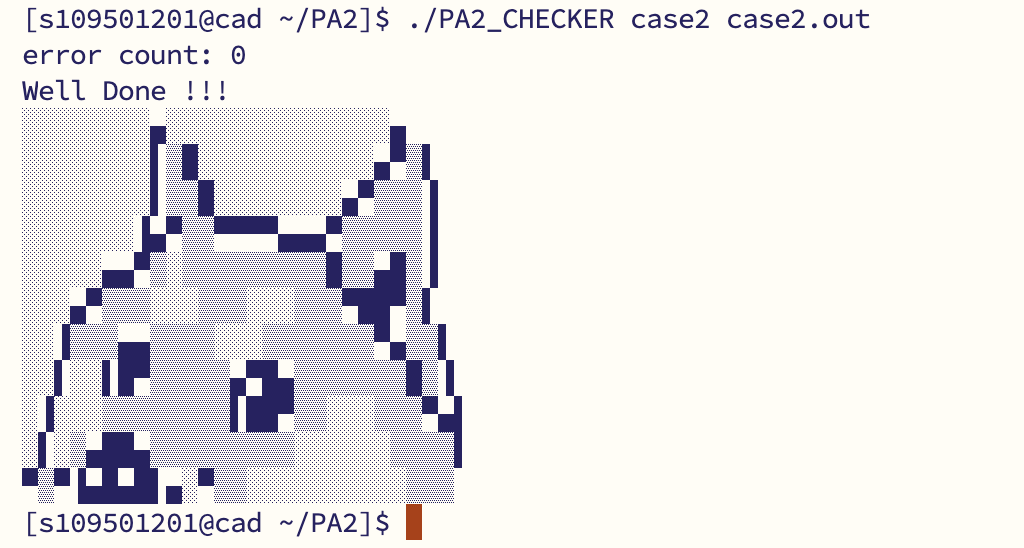
\includegraphics[width=\linewidth]{./img/2024-04-23-12-37-38.png}
  \caption{Use the executable file to ISCAS'85 netlist into Verilog format}
  \label{Checker}
\end{figure}


\pagebreak

\section{Pseudo Code}

\begin{breakablealgorithm}
  \caption{Simulated Annealing Algorithm}
  \begin{algorithmic}[1]
    \Function{SimulatedAnnealing}{}
    \State Initialize $T$ (temperature), $T_{\text{end}}$ (ending temperature), $c_{\text{now}}$ (starting configuration)
    \If{$c_{\text{now}}$ is $nullptr$}
      \State \Return
    \EndIf
    \State $c_{\text{best}}\rightarrow cut\_size \gets 0$
    \Repeat
      \Repeat
        \State Perturb($c_{\text{now}}$, $c_{\text{next}}$) \Comment{Generate a solution}
        \If{Cost($c_{\text{next}}$) $<$ Cost($c_{\text{now}}$) \textbf{and} IsConstraint1($c_{\text{next}}$)} \Comment{Compare energy}
          \State $c_{\text{now}} \gets c_{\text{next}}$
          \If{Cost($c_{\text{now}}$) $<$ Cost($c_{\text{best}}$) \textbf{and} IsConstraint1($c_{\text{now}}$)}
            \State $c_{\text{best}} \gets c_{\text{now}}$ \Comment{Accept the new solution}
          \EndIf
        \ElsIf{Metropolis($t$, Cost($c_{\text{next}}$) - Cost($c_{\text{now}}$))} 
          \State $c_{\text{now}} \gets c_{\text{next}}$ \Comment{Acceptance probability}
        \EndIf
      \Until{IsConstraint1($c_{\text{best}}$)}
      \State $T \gets alpha \times T$
    \Until{$T \leq T_{end}$} \Comment{Update temperature}
    \EndFunction
  \end{algorithmic}
\end{breakablealgorithm}


\section{PA}

\subsection{The degree of completion of the assignment: \textcolor{red}{ALL}}

\subsection{Code Explanation}

\begin{figure}[H]
\begin{lstlisting}[language = {c++},caption={Preprocessors}, label={library}]
#include <iostream> // Used for standard input-output streams
#include <map>
#include <fstream> // Used for file input-output
#include <string>
#include <sstream>
#include <vector>
#include <cmath> // Provides definitions for mathematical functions
#include <ctime> // Used for obtaining system time
#include <set>
#include <chrono> //providing representations of time points and durations
#include <iomanip> // setw
#include <limits.h> // Use the INT_MAX
\end{lstlisting}
\end{figure}
\vspace*{-1em}

According to \noindent Listing~\ref{func}, there are structures here to hold all the necessary circuit information in order to facilitate information transfer.
The ckt structure is used to store the input file information, and the ab structure is used to record the partitioning of the circuit into two sub-circuits, A and B.

\lstinputlisting[caption={Struct and Class}, label={func}, language={c++}, firstnumber=last]{./Prototype.cpp}

Following the \noindent listing~\ref{main}, I write the seeds random generator using the current time.I divide the behaviour into two branches - process file and partitioning.
 
\lstinputlisting[caption={The main function}, label={main}, language={c++}, firstnumber=last]{./main.cpp}

As indicated in Listing~\ref{inputfile}, the format file is designed to be read once. The information will be collected in its entirety during the initial pass. 

\lstinputlisting[caption={Input file process}, label={inputfile}, language={c++}, firstnumber=last]{./input_file.cpp}

As indicated in Listing~\ref{outputfile}, the output file will be generated at this location. This process would result in the outstreaming of the information stored in ABnet.

\lstinputlisting[caption={Output file process}, label={outputfile}, language={c++}, firstnumber=last]{./output_file.cpp}


In accordance with Listing~\ref{first_pass}, the search for information in the input file should commence, with the string being transformed into an integer. The nets are of the type map<int, set<int> >. The key value is the net name, while the set<int> is used to store the corresponding cells connected by the net.

\lstinputlisting[caption={First file process}, label={first_pass}, language={c++}, firstnumber=last]{./first_pass.cpp}

In accordance with Listing~\ref{count}, the total size of the net and the cell size can be determined.

\lstinputlisting[caption={Net and cell count}, label={count}, language={c++}, firstnumber=last]{./count.cpp}

In accordance with Listing~\ref{SA}, this is the method of simulated annealing (SA). Initially, the temperature is set and then decreased over time. To prevent the process from being terminated prematurely, a measurement of elapsed time is employed. The objective is to identify the optimal solution, which is believed to be provided by ABnet.

\lstinputlisting[caption={Simulated Annealing}, label={SA}, language={c++}, firstnumber=last]{./SA.cpp}

In accordance with Listing~\ref{c1}, it is necessary to ensure that the size of the A and B blocks is as uniform as possible and that the A and B blocks are present. The function would be employed in the context of both the SA and the Perturb functions.

\lstinputlisting[caption={Constraint1}, label={c1}, language={c++}, firstnumber=last]{./Constraint.cpp}

In accordance with the definition provided in Listing~\ref{M}, the objective is to return the bool in order to prevent the local optimisation.

\lstinputlisting[caption={Metropolis}, label={M}, language={c++}, firstnumber=last]{./M.cpp}

In accordance with Listing~\ref{cost}, the cut\_size is defined as the cost that should be used as the basis for determining whether the best solution or next solution should be refreshed in SA.

\lstinputlisting[caption={Cost}, label={cost}, language={c++}, firstnumber=last]{./cost.cpp}


In accordance with Listing~\ref{Perturb}, if the optimal solution (ABnet) does not have the requisite value, it is permissible to simply add the cut. Otherwise, it is necessary to perform a 10\% perturbation of the present cut and ascertain whether the perturbation would influence the constraint to the extent that it would not be satisfied. If the constraint is not satisfied, the perturbation should be recovered in order to prevent bias. 

\lstinputlisting[caption={Perturbation}, label={Perturb}, language={c++}, firstnumber=last]{./Perturb.cpp}


In accordance with Listing~\ref{SP}, use this functions to clasify the block A and B.

\lstinputlisting[caption={Start partitioning}, label={SP}, language={c++}, firstnumber=last]{./SP.cpp}

In accordance with the initial definition provided in Listing~\ref{DefineC}, this is to define the connection between cells following a cut.

\lstinputlisting[caption={Define connections of the cells}, label={DefineC}, language={c++}, firstnumber=last]{./DefineC.cpp}

In accordance with the definition provided in Listing~\ref{Find}, the objective is to implement DFS to accurately define the relationship between cells following a cut.

\lstinputlisting[caption={Find the connection between cells}, label={Find}, language={c++}, firstnumber=last]{./Find.cpp}

In accordance with the definition provided in Listing~\ref{ab}, it can be demonstrated that there are some independent blocks other than A or B, and that they can be added into A or B.

\lstinputlisting[caption={To merge the other block into A or B}, label={ab}, language={c++}, firstnumber=last]{./AB.cpp}

In accordance with the definition provided in Listing~\ref{IsFind}, the objective is to ascertain the existence of the cell in either the A or B block.

\lstinputlisting[caption={Find the cell in A or B}, label={IsFind}, language={c++}, firstnumber=last]{./IsFind.cpp}

In accordance with the definition provided in Listing [S], the function is to prevent the incorrect cut-size.

\lstinputlisting[caption={Shrink the redundant cut}, label={S}, language={c++}, firstnumber=last]{./Shrink.cpp}

\pagebreak
% ------------------------------
\section{The hardness of this assignment / I overcome it}

\begin{enumerate}
    \item Segmentation fault when pointer to the struct contain container such as set and vector.\\
    Ans: If there are vector, set or map in structure, it should be allocate information or give their Initialization. Otherwise, it would cause segmentation. And before searching the container, it would recommand to check it is not empty. \\\href{https://blog.csdn.net/little_girl_ly/article/details/80634906?spm=1001.2101.3001.6650.1&utm_medium=distribute.pc_relevant.none-task-blog-2%7Edefault%7ECTRLIST%7ERate-1-80634906-blog-39520113.235%5Ev43%5Epc_blog_bottom_relevance_base3&depth_1-utm_source=distribute.pc_relevant.none-task-blog-2%7Edefault%7ECTRLIST%7ERate-1-80634906-blog-39520113.235%5Ev43%5Epc_blog_bottom_relevance_base3&utm_relevant_index=2}{C++结构体中包含容器push\_back异常}\\\href{https://blog.csdn.net/jinking01/article/details/117082102}{使用带map容器的struct结构体指针引发的段错误}

    \item Makefile missing separator. Stop.\\
    Ans: Set tabstop = 4 
    

\end{enumerate}

% ------------------------------

\section{Suggestions}

No.

\end{document}